\documentclass{beamer}
%математика
\usepackage{amssymb,amsmath,mathtext}
\usepackage{indentfirst,amsfonts}
\usepackage{makecell,multirow,longtable}
%язык
\usepackage[english,russian]{babel}
\usepackage[utf8]{inputenc}
% Стиль презентации
\usetheme{Warsaw}
\useoutertheme{infolines}
\begin{document}
\title[Линейные и нелинейные модели]{Линейные и нелинейные модели в задачах автоматической классификации текстов на естественных языках}  
\author[Бочаров И.А.]{Бочаров И.А., А-13-08 \\Научный руководитель: д.т.н., проф. Фальк В.Н.,\\Консультант: Шаграев А.Г.}

\institute{НИУ МЭИ, АВТИ, Кафедра Прикладной математики}
\date{Москва, 2014} 
% Создание заглавной страницы
\begin{frame}[plain]
	\titlepage
\end{frame}
% Автоматическая генерация содержания
\begin{frame}
	\tableofcontents
\end{frame}


\section{Постановка задачи классификации}
\begin{frame}
\frametitle{Постановка задачи классификации}
Пусть $X$ - множество классифицируемых объектов, а $Y$ - конечное множество классов. Имеется целевая функция - отображение $y^*:X\rightarrow Y$, значения которой известны только на конечном подмножестве объектов $X' \subset X$ обучающей выборки \\
$$X^l=\{\langle x_i,y_i \rangle |x_i \in X', y_i=y^*(x_i),1\le i \le l\}$$
Необходимо построить решающую функцию $a: X \rightarrow Y$ , принадлежащую
некоторому классу функций $\theta$, которая была бы как можно более качественным
приближением к целевой функции. 
\\Методом обучения $\mu$ будем называть функцию, ставящую в соответствие любой обучающей выборке некоторую
решающую функцию из класса $\theta: \mu(X^l)=a \in \theta$
\end{frame}

\section{Оценка качества классификации}
\begin{frame}
\frametitle{Оценка качества классификации}
Для измерения качества предсказаний необходимо определить функционал
качества – функцию, которая всякому набору прецедентов (пар, состоящих из
объектов и соответствующих им ответов) и решающей функции сопоставляет
некоторое число. Считается, что, чем больше значение функционала качества, тем лучше качество предсказаний решающей функции.
\newline
\newline
\newline
Пусть $X^t$-тестовая выборка. Тогда значение функционала $$Q(X^t,\mu(X^l))$$ можно считать оценкой обобщающей способности метода обучения $\mu$.
\end{frame}

\subsection{Скользящий контроль}
\begin{frame}
\frametitle{Скользящий контроль}
	Пусть имеется обучающая выборка $X^l$, метод обучения $\mu$ и некоторый функционал качества $Q$. Зафиксируем множество разбиений выборки $X^l$:
	$$\{\{S_1^l,S_1^t\},\{S_2^l,S_2^t\},...,\{S_k^l,S_k^t\}\},$$
	$$S_i^l \cup S_i^t = X^l, i=1..k$$
	Оценка качества, усредненная по всем разбиениям, называется оценкой скользящего контроля:
	$$CV(Q,\mu,S)=\frac{1}{k}\sum\limits_{i=1}^{k}Q(S_i^t,\mu(S_i^l))$$
\end{frame}

\begin{frame}
\frametitle{Стратификация выборки}
	Желательно, чтобы разбиения, используемые при получении оценок методом скользящего контроля обладали теми же статистическими свойствами, что и вся выборка $X^l$. Для достижения этого часто используется стратификация.
	\newline
	\newline
	Стратификация классов заключается в том, что разбиения проводятся таким образом, что доля каждого класса $k$ в каждой подвыборке $X_i^l$ примерно равна:
	$$\frac{|X_i^l|}{|X^l|}\sum\limits_{\langle x,y \rangle \in X^l}^{}[y=k],$$
	где:\\
	\begin{equation*}
	[X]=
	\begin{cases}
	&1, если\ условие\ X\ выполняется,\\
	&0, в\ противном\ случае.
	\end{cases}
	\end{equation*}
\end{frame}

\section{Методы классификации}
\subsection{Логистическая регрессия}
\begin{frame}
\frametitle{Логистическая регрессия}
При использовании метода логистичекой регрессии строится линейный алгоритм вида
$$a(x,\omega)=sign\left(\sum\limits_{i=1}^M\omega_j x_j-\omega_0\right)=sign\left(\langle x,\omega \rangle\right),$$ где $\langle x,\omega \rangle$ - скалярное произведение векторов $x$ и $\omega$.
\newline
\newline
Задача обучения логистической регрессии сводится к настройке вектора весов $\omega\in \mathbb{R}^M$ по выборке $X^l$.
\end{frame}

\begin{frame}
\frametitle{Обучение логистической регрессии}
Задача обучения логистической регрессии решается при помощи метода минимизации эмпирического риска с функцией потерь следующего вида:
$$Q(\omega, X^l)=\sum\limits_{i=1}^l ln(1+exp(-y_i\langle x_i,\omega \rangle))\rightarrow \min\limits_{\omega}$$
Вычислим частные производные функции потерь:
$$\frac{\partial Q}{\partial \omega_j}=\sum\limits_{y^*(x_i)=+1}\frac{x_{ij}}{1+exp(\langle x_i,\omega\rangle)}+\sum\limits_{y^*(x_i)=-1}\frac{-x_{ij}}{1+exp(\langle x_i,\omega\rangle)}$$
Получение явных выражений для величин $\omega_j$ из условий $\frac{\partial Q}{\partial \omega_j}=0, j=1..M$ к сожалению, невозможно. Для получения приближенного решения задачи используется метод стохастического градиентного спуска.
\end{frame}

\begin{frame}
\frametitle{Модификации метода логистической регрессии}
\begin{itemize}
	\item{Стратификация\newline 
		На каждом шаге метода стохастического градиентного спуска используются два объекта – один,
		принадлежащий положительному классу, а второй – отрицательному.
	}
	\item{Модификация функционала потерь}
\end{itemize}
\end{frame}

\begin{frame}
\frametitle{Модификация функционала потерь метода логистической регрессии}
	Введем смещения в функционал потерь:
	$$Q(\omega, X^l)=\sum\limits_{i=1}^l ln(1+exp(-y_i\langle x_i,\omega \rangle +c))\rightarrow \min\limits_{\omega}$$
	Изменятся и значения частных производных:
	$$\frac{\partial Q}{\partial \omega_j}=\sum\limits_{y^*(x_i)=+1}\frac{x_{ij}}{1+exp(\langle x_i,\omega\rangle +c)}+\sum\limits_{y^*(x_i)=-1}\frac{-x_{ij}}{1+exp(\langle x_i,\omega\rangle +c)}$$
	Параметр $c$ становится параметром метода и может быть выбран, к примеру, на основе скользящего контроля.
\end{frame}

\begin{frame}
\frametitle{Положительный эффект от введения смещений}
Приведем ответы решающего правила без использования смещений и с использованием смещений.
 \begin{columns}[T]
    \begin{column}{.5\textwidth}
    \begin{block}{Без использования смещений}
% Your image included here
    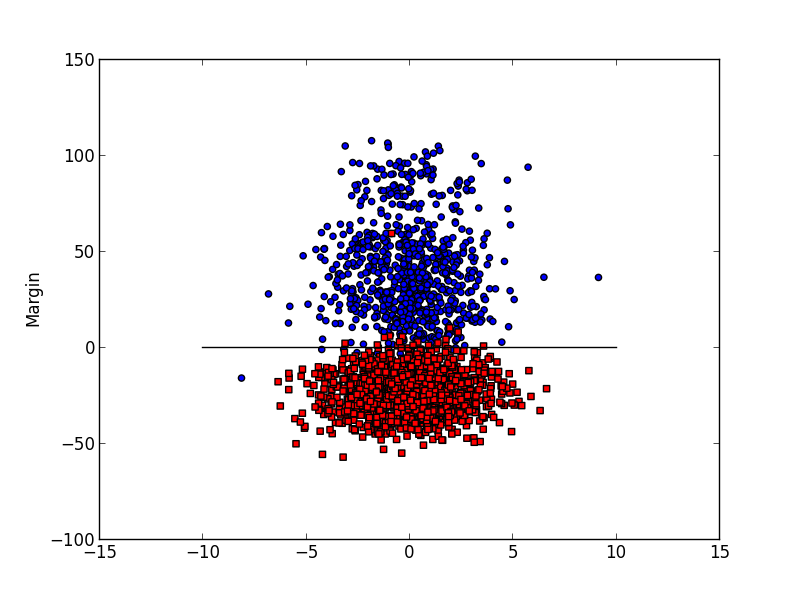
\includegraphics[width=\linewidth,height=\textheight,keepaspectratio]{/home/bocharov-ivan/Presentation/master-presentation/1.png}
    \end{block}
    \end{column}
    \begin{column}{.5\textwidth}
    \begin{block}{С использованием смещений}
% Your image included here
    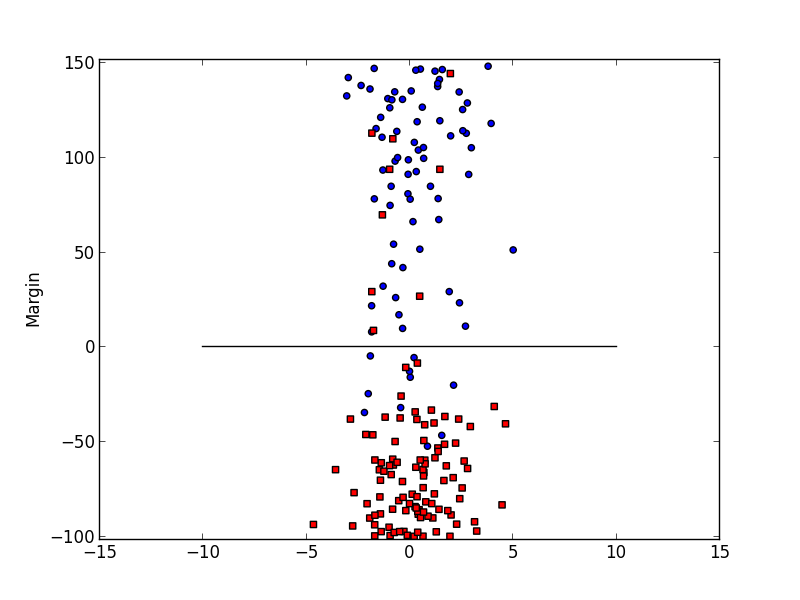
\includegraphics[width=\linewidth,height=\textheight,keepaspectratio]{2.png}
    \end{block}
    \end{column}
  \end{columns}
Приведенные результаты позволяют судить, что использование смещений приводит к более уверенной классификации.
\end{frame}


\subsection{k ближайших соседей}
\begin{frame}
\frametitle{Построение метода}
Пусть на множестве $X$ введена коммутативная функция расстояния $\rho:X\times X\rightarrow[0,+\infty)$. В этом случае возможно построение разнообразных метрических методов.\\
Для произвольного $u\in X^l$ расположим элементы обучающей выборки в порядке возрастания расстояний до $u$:
$$\rho(u,x_u^{(1)})\le\rho(u,x_u^{(2)})\le ... \le \rho(u, x_u^{(l)})$$
Пусть $y_u^{(i)}=a(x_u^{(i)})$. Во введенных обозначениях решающее правило метода $k$ ближайших событий принимает вид $$a(u; X^l, k)=\arg\max\limits_{y \in Y}\sum\limits_{i=1}^{k}[y_u^{(i)}=y]$$
\end{frame} 

\begin{frame}
\frametitle{Введение весовых коэффициентов}
Максимум в решающем правиле метода $k$ ближайших соседей может достигаться на нескольких классах. Чтобы избежать неоднозачности, вводится строго убывающая последовательность весов $\omega_i$, задающих вклад $i$-го соседа в классификацию:
$$a(u; X^l, k)=\arg\max\limits_{y \in Y}\sum\limits_{i=1}^{k}[y_u^{(i)}=y]\omega_i$$
При использовании в качестве весов геометрической прогрессии $\omega_i=q^i, q\in(0;1)$ неоднозначностей удается гарантированно избежать.
\end{frame} 

\section{Сокращение размерности признакового пространства}

\begin{frame}
\frametitle{Методы сокращения размерности}
\begin{itemize}
	\item{Отбор признаков}
		\begin{itemize}
		\item{Полный перебор}
		\item{Последовательное добавление/удаление признаков}
		\item{Кластеризация признаков}
		\item{Генетические алгоритмы}
		\end{itemize}
	\item{Синтез признаков}
		\begin{itemize}
		\item{Метод главных компонент, PCA}
		\item{Нейросетевой подход к синтезу признаков}
		\end{itemize}
\end{itemize}
\end{frame}

\begin{frame}
\frametitle{Разреженный автоэнкодер(spatial autoencoder)}
\begin{columns}[T]
    \begin{column}{.5\textwidth}
    \begin{block}{Структура автоэнкодера}
    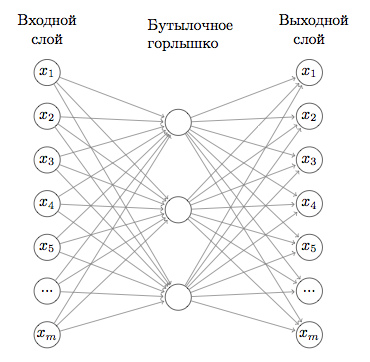
\includegraphics[width=\linewidth,height=.7\textheight,keepaspectratio]{/home/bocharov-ivan/Presentation/master-presentation/autoencoder.png}
    \end{block}
    \end{column}
  \end{columns}
\end{frame}

\begin{frame}
\frametitle{Модификация автоэнкодера}
\begin{columns}[T]
    \begin{column}{.5\textwidth}
    \begin{block}{Структура модифицированного автоэнкодера}
    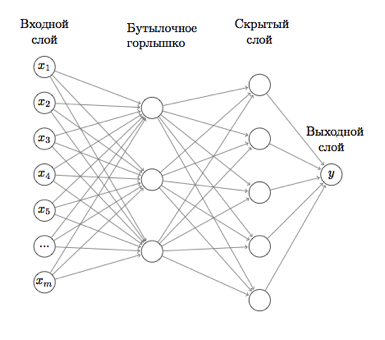
\includegraphics[width=\linewidth,height=.7\textheight,keepaspectratio]{/home/bocharov-ivan/Presentation/master-presentation/modified_encoder.png}
    \end{block}
    \end{column}
  \end{columns}
\end{frame}

\section{Вычислительные эксперименты}
\begin{frame}
\frametitle{Эксперимент №1}
\end{frame}

\section{}
\begin{frame}
\frametitle{Спасибо за внимание!}
	Спасибо за внимание!
\end{frame}

\end{document}
